\chapter{\label{ch:exp_work}Implementation and Experimental Evaluations}
\markright{Mohammed El-Shambakey \hfill Chapter~\ref{ch:exp_work}. Experiments \hfill}
%
Having established upper bounds for retry cost and response time of different contention managers, and the conditions under which each one is preferred. We now would like to understand how each CM retries in practice (i.e., on average) compared with that of competitor methods. Since this can only be understood experimentally, we implement ECM, RCM, LCM, PNF, FBLT, OMLP, RNLP and lock-free and conduct experimental studies.

The rest of this Chapter is organized as follow: Section~\ref{sec:methodology} outlines the used methodology to generate different tasksets and run experiments. Section~\ref{sec:exp_tasksets_properties} outlines properties of used task sets and atomic sections for comparing different contention managers, locking protocols and lock-free. Section~\ref{sec:performance_measurements} presents used metrics to evaluate performance of different synchronization techniques. Section~\ref{sec:final_results} discusses experimental results.
%
\section{Methodology}\label{sec:methodology}
%
We used the ChronOS real-time Linux kernel~\cite{dellinger2011chronos}
and the RSTM library~\cite{marathe2006lowering}. We modified RSTM to include implementations of ECM, RCM, LCM, PNF and FBLT contention managers, and modified ChronOS to include implementations of G-EDF and G-RMA schedulers and Global OMLP\cite{springerlink:10.1007/s10617-012-9090-1,key-3} and RNLP\cite{6257574} locking protocols. For the retry-loop lock-free implementation, we used a loop that reads an object and attempts to write to the object using a compare-and-swap (CAS) instruction. The task retries until the CAS succeeds. We use an 8 core, 2GHz AMD Opteron platform.

Experiments ran over a set of tasksets. Each taskset consists of a number of tasks. Each task is represented by a single thread. Our system assumes sporadic task model. However, to simplify experiments and enable comparison between different synchronization techniques, we used implicit periodic tasks where relative deadline equals period of each task. The least common multiplier of periods of all tasks in a single taskset is called \textit{Hyperperiod} of this taskset. Each task $\tau_i$ in a single taskset runs a number of jobs(i.e., instances) equal to hyperperiod of the taskset divided by period of the task, $T_i$.
%
\section{Tasksets}\label{sec:exp_tasksets_properties}
%
We collected properties of tasksets from~\cite{6001644,6064513,brandenburg2008comparison,key-4,bc+08,5161514,
springerlink:10.1007/s11241-010-9097-2,springerlink:10.1007/s10617-012-9090-1,
lakshmanan2009coordinated,4700432,Baker05acomparison,lindsay2012lwfg} with some modifications due to insertion of transactions into tasks. Each task's period, $T_i$, is an integer uniformly distributed from $[10ms,100ms]$. Utilization of each task, $u_i$, is derived from three uniform distributions: $[0.001,0.1]$ (light), $[0.1,0.4]$ (medium), and $[0.5,0.9]$(heavy). Worst case execution time for each task, $e_i$, is calculated as $e_i=u_i.T_i$. Total utilization of all tasks in a given specific taskset should not exceed $\hat{U}$. Different tasksets are generated for each $\hat{U} \in \{2,4,6,8\}$ where 8 is the maximum number of cores on the tested platform as given in Section~\ref{sec:methodology}. Tasks are added to each taskset until $\hat{U}$ is reached. If last task makes total utilization exceeds $\hat{U}$, then the last task is removed.

Each task has a number of atomic sections(transactions). Atomic section properties are probabilistically controlled using three parameters: the maximum($max_{Tx}$) and minimum($min_{Tx}$) lengths of any atomic section within the task, and the total($to_{Tx}$) length of atomic sections within any task. Each of the 3 parameters ($min_{Tx}$,$max_{Tx}$ and $to_{Tx}$) is derived from 3 uniform distributions: $[0,0.3)$ (light), $[0.3,0.6)$ (medium), $[0.6,1]$ (heavy). Each value of $min_{Tx}$,$max_{Tx}$ and $to_{Tx}$ is relative to $e_i$. Thus, each of $min_{Tx}$,$max_{Tx}$ and $to_{Tx}$ does not exceed $e_i$. $max_{Tx}$ is chosen such that $max_{Tx} \le to_{Tx}$. Similarly, $min_{Tx}$ is chosen such that $min_{Tx} \le max_{Tx}$. Total number of shared objects, $N^r$, is 40. Number of objects per each atomic section, $N_i^r$, is chosen from 3 uniform distributions: $[0,0.3)$ (light), $[0.3,0.6)$ (medium), $[0.6,1]$ (heavy). As lock-free cannot access more than one object in one atomic operation, tasks share one object per transaction when lock-free is included in comparison. Different properties for tasks and transactions are summarized in Table~\ref{table:taskset_properties}.
%
\begin{flushleft}
\begin{table}[htbp]
\begin{centering}
\caption{\label{table:taskset_properties}Tasksets' and transactions' properties}
\begin{tabular}{|c|>{\raggedright}p{14cm}|}
\hline 
$\hat{U}$ & $\{2,4,6,8\}$\tabularnewline
\hline 
$T_{i}$ & uniformly chosen from $[10ms,100ms]$\tabularnewline
\hline 
$u_{i}$ & Uniformly chosen from $[0.001,0.1]$ (light), $[0.1,0.4]$ (medium),
and $[0.5,0.9]$(heavy). $\sum_{\forall i}u_{i}\le\hat{U}$\tabularnewline
\hline 
$e_{i}$ & $u_{i}.T_{i}$\tabularnewline
\hline 
$to_{Tx}$ & Uniformly chosen from $[0,0.3)$ (light), $[0.3,0.6)$ (medium), $[0.6,1]$
(heavy) relative to $e_{i}$\tabularnewline
\hline 
$max_{Tx}$ & Uniformly chosen from $[0,0.3)$ (light), $[0.3,0.6)$ (medium), $[0.6,1]$
(heavy) relative to $e_{i}$. $max_{Tx}\le to_{Tx}$\tabularnewline
\hline 
$min_{Tx}$ & Uniformly chosen from $[0,0.3)$ (light), $[0.3,0.6)$ (medium), $[0.6,1]$
(heavy) relative to $e_{i}$. $min_{Tx}\le max_{Tx}$\tabularnewline
\hline 
$N^{r}$ & 40\tabularnewline
\hline 
$N_{i}^{r}$ & Uniformly chosen from $(0,0.3)$ (light), $[0.3,0.6)$ (medium), $[0.6,1]$
(heavy)\tabularnewline
\hline 
\end{tabular}
\par\end{centering}
\end{table}
\par\end{flushleft}
%
\section{Performance Measurements}\label{sec:performance_measurements}
%
MENTION DSR, TARDINESS FROM MATHEW'S THESIS. ADD RC AND DIFFERENTIATE BETWEEN FIRST INSTANCE AND OTHERS
%
\section{Results}\label{sec:final_results}
%
Figure~\ref{fig:pnf_results_1_obj_all} shows average retry cost under ECM, RCM, LCM, PNF and lock-free for each task set. Figure~\ref{fig:pnf_results_1_obj_without_lock_free} shows average retry cost for only contention managers for each task set. The $x$-axis has three parameters $a,b,c$. $a$ specifies the relative total length of all atomic sections to the length of the task. $b$ specifies the maximum relative length of any atomic section to the length of the task. $c$ specifies the minimum relative length of any atomic section to the length of the task. Each data point in the figure has a confidence level of 0.95.
Only one object per transaction is shared in Figures~\ref{fig:pnf_results_1_obj_all} and~\ref{fig:pnf_results_1_obj_without_lock_free}.

Lock-free is the longest technique as it provides no conflict resolution. PNF better or comparable retry cost than ECM, RCM and LCM. As we move from 4 to 8 to 20 task set, retry costs of different contention managers get closer to each other. This is explained by noting that each task set in Table~\ref{pnf_task_sets_table} is organized in non-decreasing order of periods, and $c_i/T_i$ for almost each $\tau_i$ is low. Besides, each task shares objects only with the previous and next tasks, and tasks are released at the same time to enforce transitive retry. While the first instances of all tasks have a high potential of conflict, the contention level decreases with time for higher number of tasks. Thus, for the 20 task set, contention level is the lowest. Hence, retry costs of all contention managers get closer as number of tasks increases.

We compared retry cost for different contention managers with multiple objects per transaction and different levels of read/writer operations. Figure~\ref{fig:cm_20obj_per_tx_40wr} shows retry cost of the three task sets sharing 20 objects per transaction, with 40\% write operations and 60\% read operations. The same experiment is repeated in Figure~\ref{fig:cm_20obj_per_tx_80wr} with 80\% write operations, and 20\% read operations. Figure~\ref{fig:cm_20obj_per_tx_100wr} repeats the same experiment with 100\% write operations. The same previous three experiments were repeated in Figures~\ref{fig:cm_40obj_per_tx_40wr},~\ref{fig:cm_40obj_per_tx_80wr} and~\ref{fig:cm_40obj_per_tx_100wr} with 40 objects per transaction. Figures~\ref{fig:cm_20obj_per_tx_40wr} to~\ref{fig:cm_40obj_per_tx_100wr} show consistent trends with Figure~\ref{fig:pnf_results_1_obj_without_lock_free} except that retry cost of PNF is shorter than the others even with increasing number of tasks. For the 20 task set, PNF retry cost is a little shorter than LCM, but much better than ECM and RCM. This happens because of sharing multiple objects per transaction. Thus, contention level is increased than in sharing 1 object per transaction. Besides, transitive retry exists which makes PNF better than the others.
%%%%%%%%%%%%%%%%%%%%%%%%%%%%%%%%%%%%%%%%%%%%%%%%%%%%%%%

\begin{figure}
\centering

\subfigure[4 tasks]{
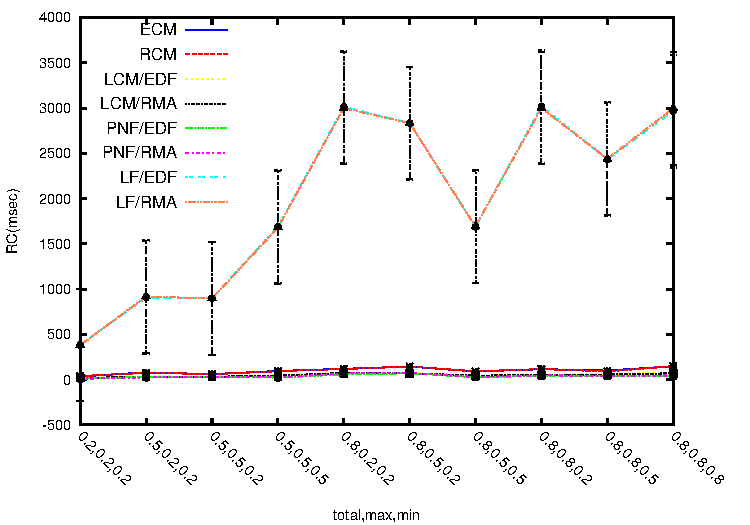
\includegraphics[scale=0.7]
{figures/Abr_dur_4t_5obj_all_100wr}
\label{fig:results_1_obj_all_4_tasks}
}
~
\subfigure[8 tasks]{
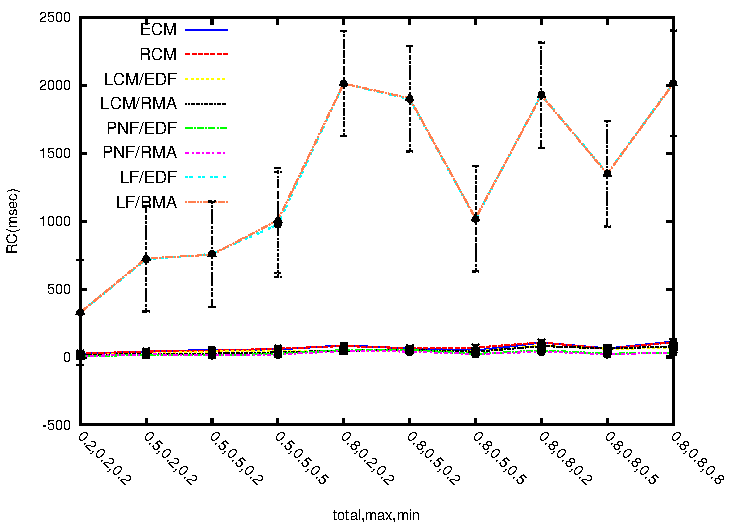
\includegraphics[scale=0.7]
{figures/Abr_dur_8t_9obj_all_100wr}
\label{fig:results_1_obj_all_8_tasks}
}
~
\subfigure[20 tasks]{
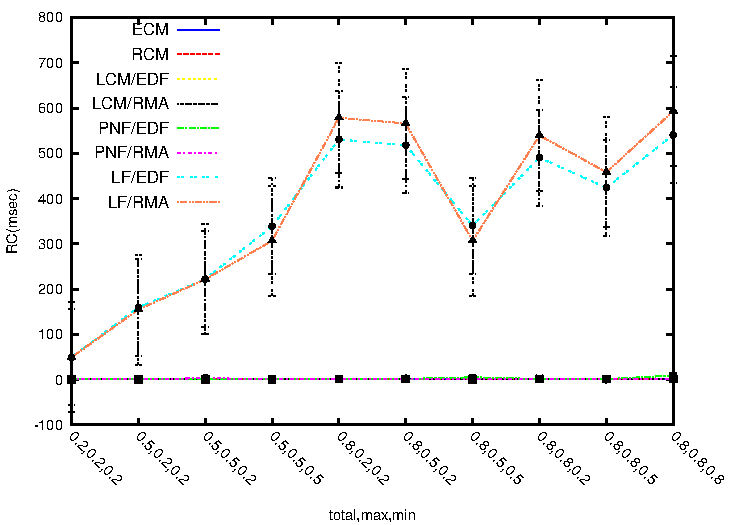
\includegraphics[scale=0.7]
{figures/Abr_dur_20t_21obj_all_100wr}
\label{fig:results_1_obj_all_20_tasks}
}
\caption{Average retry cost for 1 object per transaction for different values of total, maximum and minimum atomic section length under all synchronization techniques}
\label{fig:pnf_results_1_obj_all}
\end{figure}

\begin{figure}
\centering

\subfigure[4 tasks]{
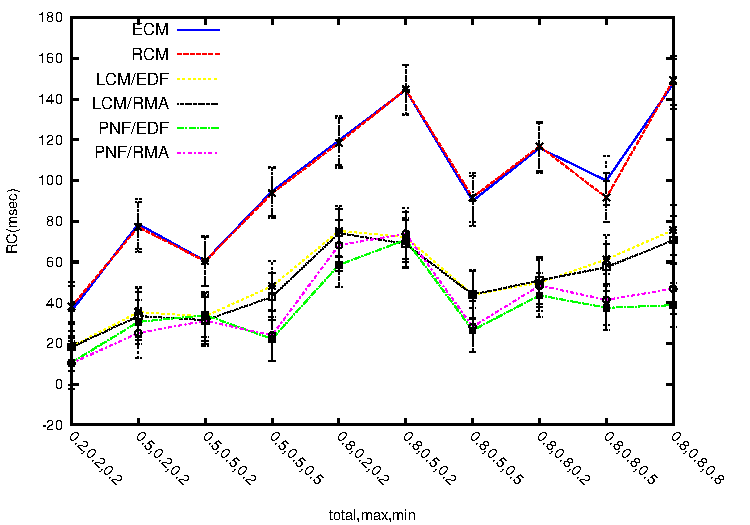
\includegraphics[scale=0.7]
{figures/Abr_dur_4t_5obj_100wr}
\label{fig:pnf_results_1_obj_cm_4t}
}
~
\subfigure[8 tasks]{
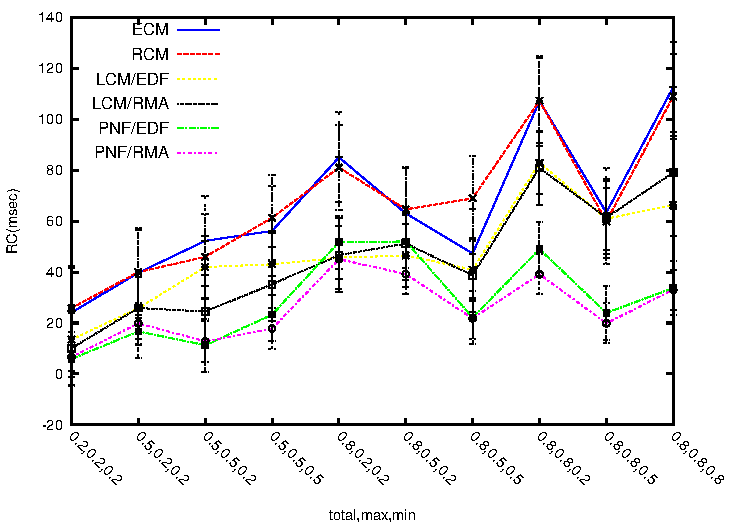
\includegraphics[scale=0.7]
{figures/Abr_dur_8t_9obj_100wr}
\label{fig:pnf_results_1_obj_cm_8t}
}
~
\subfigure[20 tasks]{
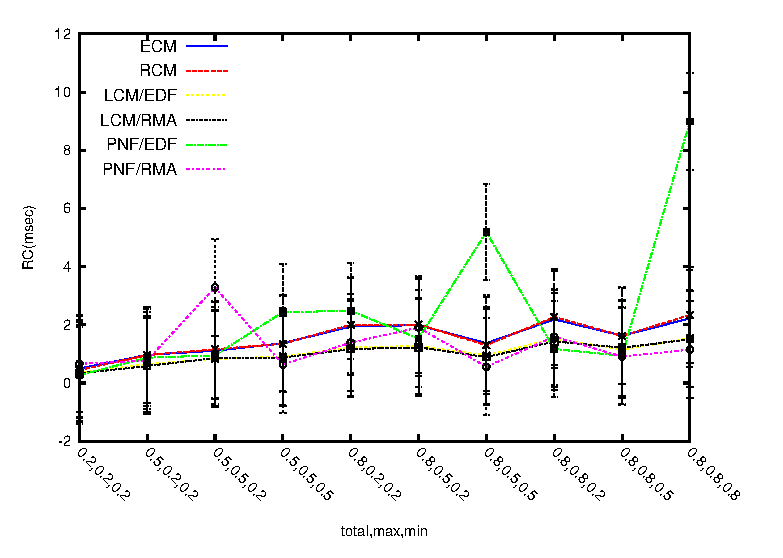
\includegraphics[scale=0.7]
{figures/Abr_dur_20t_21obj_100wr}
\label{fig:pnf_results_1_obj_cm_20t}
}
\caption{Average retry cost for 1 object per transaction for different values of total, maximum and minimum atomic section length under contention managers only}
\label{fig:pnf_results_1_obj_without_lock_free}
\end{figure}
%%%%%%%%%%%%%%%%%%%%%%%%%%%%%%%%
\begin{figure}
\centering

\subfigure[4 tasks]{
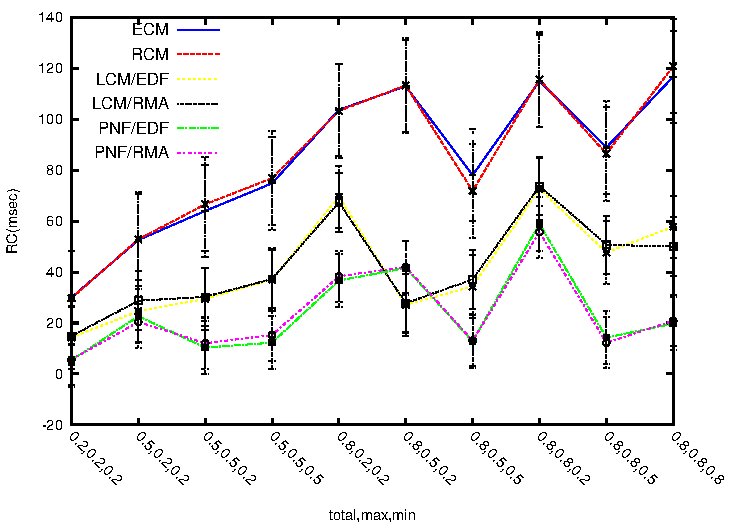
\includegraphics[scale=0.7]
{figures/Abr_dur_4t_50obj_40wr}
\label{fig:4t_ecm_rcm_lcm_pnf_50obj_40wr}
}
~
\subfigure[8 tasks]{
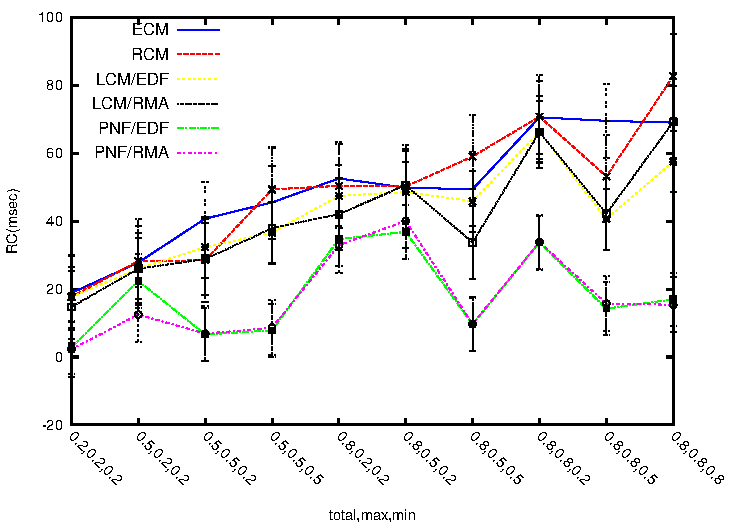
\includegraphics[scale=0.7]
{figures/Abr_dur_8t_90obj_40wr}
\label{fig:8t_ecm_rcm_lcm_pnf_90obj_40wr}
}
~
\subfigure[20 tasks]{
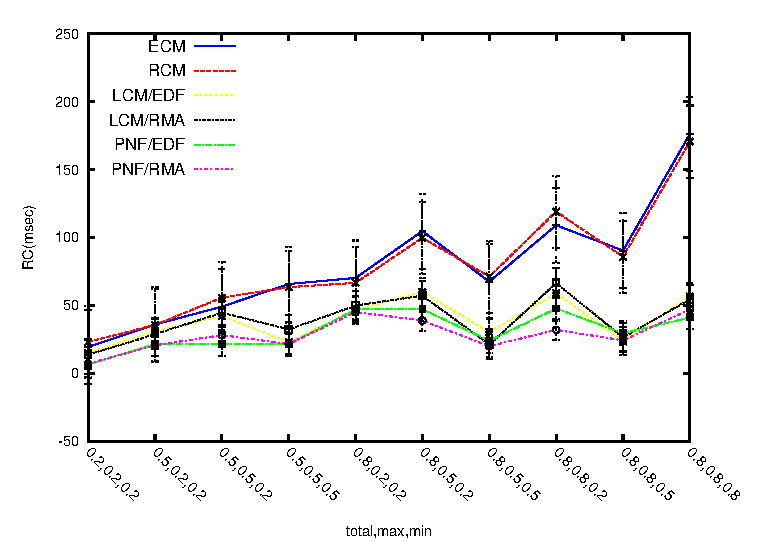
\includegraphics[scale=0.7]
{figures/Abr_dur_20t_210obj_40wr}
\label{fig:20t_ecm_rcm_lcm_pnf_210obj_40wr}
}
\caption{Average retry cost for 20 objects per transaction, 40\% write operations for different values of total, maximum and minimum atomic section length under different CMs}
\label{fig:cm_20obj_per_tx_40wr}
\end{figure}
%%%%%%%%%%%%%%%%%%%%%%%%%%%%%%%%%%%%%%%%%%%%%%%%%%%%%%
%%%%%%%%%%%%%%%%%%%%%%%%%%%%%%%%
\begin{figure}
\centering

\subfigure[4 tasks]{
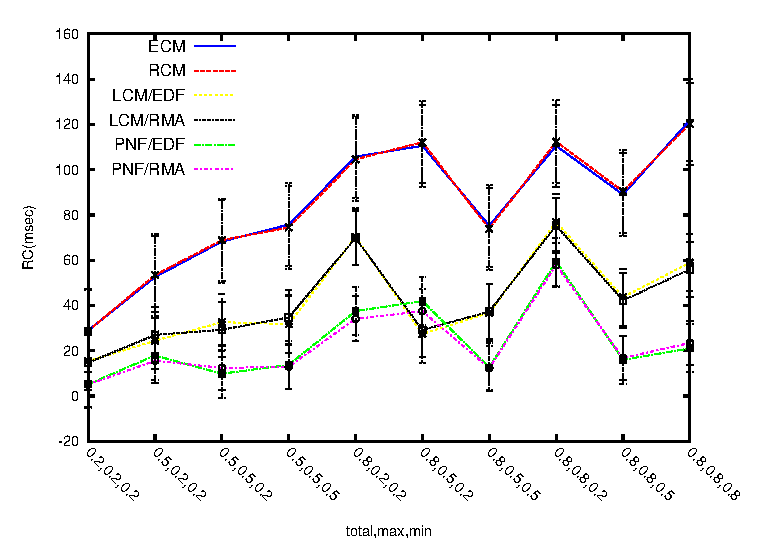
\includegraphics[scale=0.7]
{figures/Abr_dur_4t_50obj_80wr}
\label{fig:4t_ecm_rcm_lcm_pnf_50obj_80wr}
}
~
\subfigure[8 tasks]{
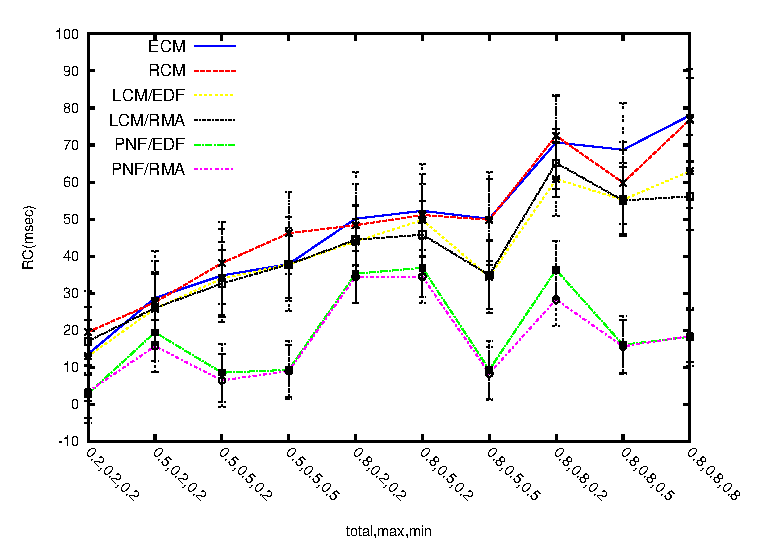
\includegraphics[scale=0.7]
{figures/Abr_dur_8t_90obj_80wr}
\label{fig:8t_ecm_rcm_lcm_pnf_90obj_80wr}
}
~
\subfigure[20 tasks]{
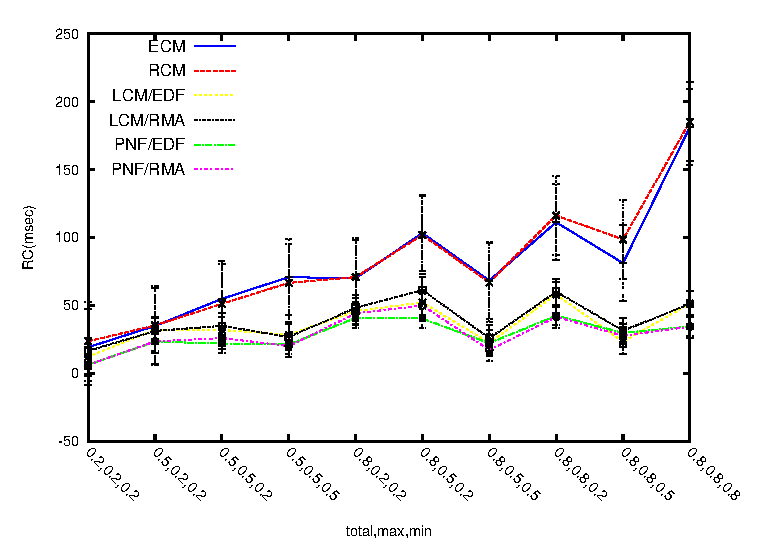
\includegraphics[scale=0.7]
{figures/Abr_dur_20t_210obj_80wr}
\label{fig:20t_ecm_rcm_lcm_pnf_210obj_80wr}
}
\caption{Average retry cost for 20 objects per transaction, 80\% write operations for different values of total, maximum and minimum atomic section length under different CMs}
\label{fig:cm_20obj_per_tx_80wr}
\end{figure}
%%%%%%%%%%%%%%%%%%%%%%%%%%%%%%%%%%%%%%%%%%%%%%%%%%%%%%
\begin{figure}
\centering

\subfigure[4 tasks]{
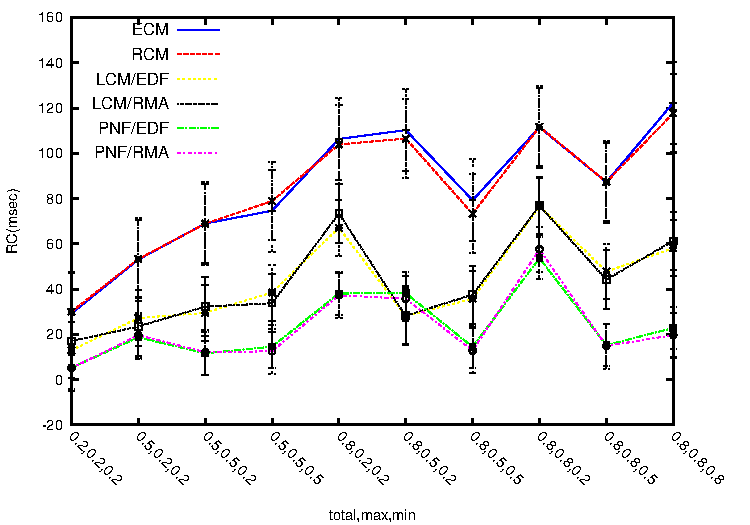
\includegraphics[scale=0.7]
{figures/Abr_dur_4t_50obj_100wr}
\label{fig:4t_ecm_rcm_lcm_pnf_50obj_100wr}
}
~
\subfigure[8 tasks]{
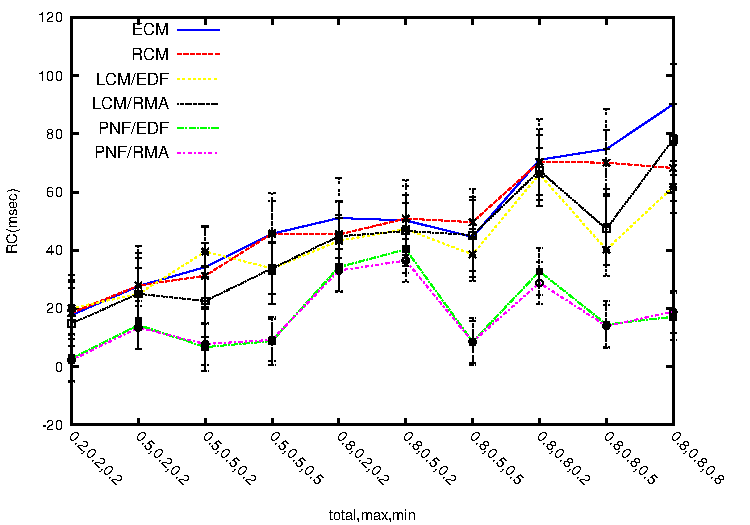
\includegraphics[scale=0.7]
{figures/Abr_dur_8t_90obj_100wr}
\label{fig:8t_ecm_rcm_lcm_pnf_90obj_100wr}
}
~
\subfigure[20 tasks]{
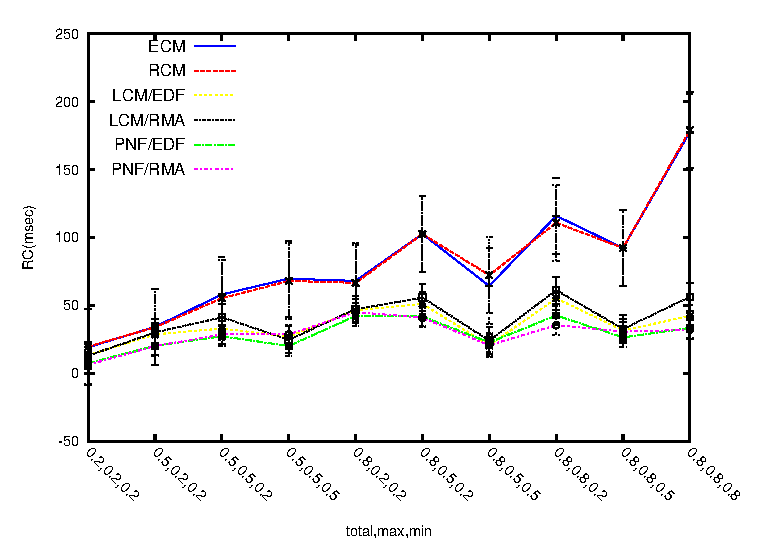
\includegraphics[scale=0.7]
{figures/Abr_dur_20t_210obj_100wr}
\label{fig:20t_ecm_rcm_lcm_pnf_210obj_100wr}
}
\caption{Average retry cost for 20 objects per transaction, 100\% write operations for different values of total, maximum and minimum atomic section length under different CMs}
\label{fig:cm_20obj_per_tx_100wr}
\end{figure}
%%%%%%%%%%%%%%%%%%%%%%%%%%%%%%%%%%%%%%%%%%%%%%%%%%%%%%
\begin{figure}
\centering

\subfigure[4 tasks]{
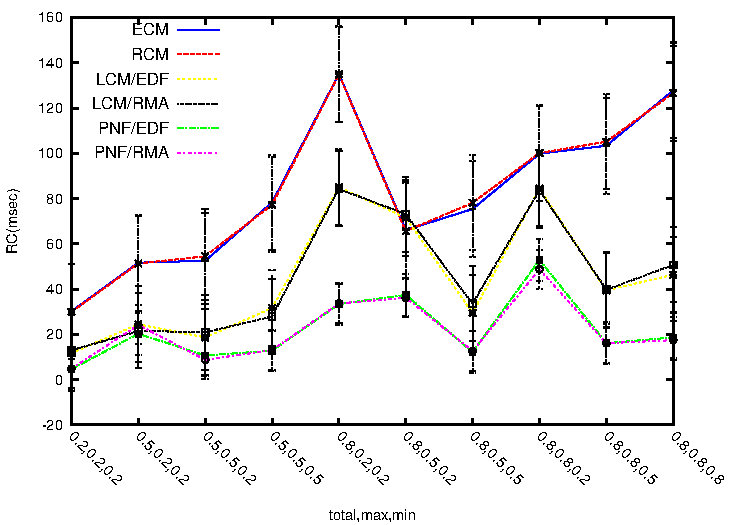
\includegraphics[scale=0.7]
{figures/Abr_dur_4t_100obj_40wr}
\label{fig:4t_ecm_rcm_lcm_pnf_100obj_40wr}
}
~
\subfigure[8 tasks]{
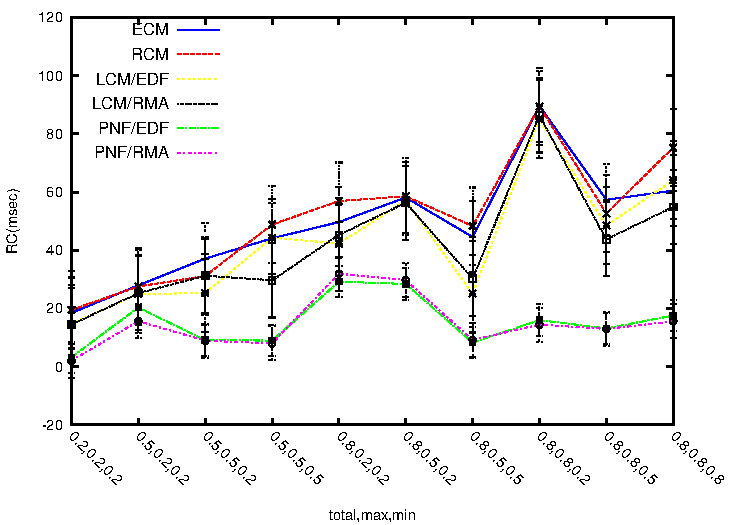
\includegraphics[scale=0.7]
{figures/Abr_dur_8t_180obj_40wr}
\label{fig:8t_ecm_rcm_lcm_pnf_180obj_40wr}
}
~
\subfigure[20 tasks]{
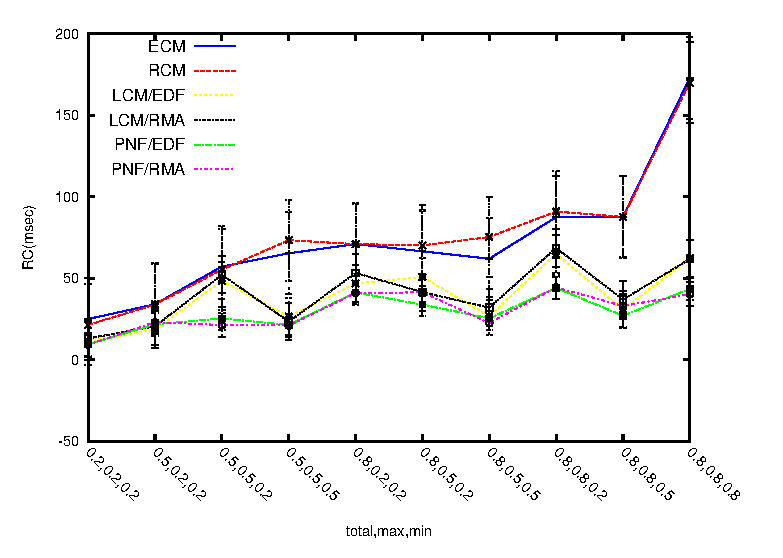
\includegraphics[scale=0.7]
{figures/Abr_dur_20t_420obj_40wr}
\label{fig:20t_ecm_rcm_lcm_pnf_420obj_40wr}
}
\caption{Average retry cost for 40 objects per transaction, 40\% write operations for different values of total, maximum and minimum atomic section length under different CMs}
\label{fig:cm_40obj_per_tx_40wr}
\end{figure}
%%%%%%%%%%%%%%%%%%%%%%%%%%%%%%%%%%%%%%%%%%%%%%%%%%%%%%
\begin{figure}
\centering

\subfigure[4 tasks]{
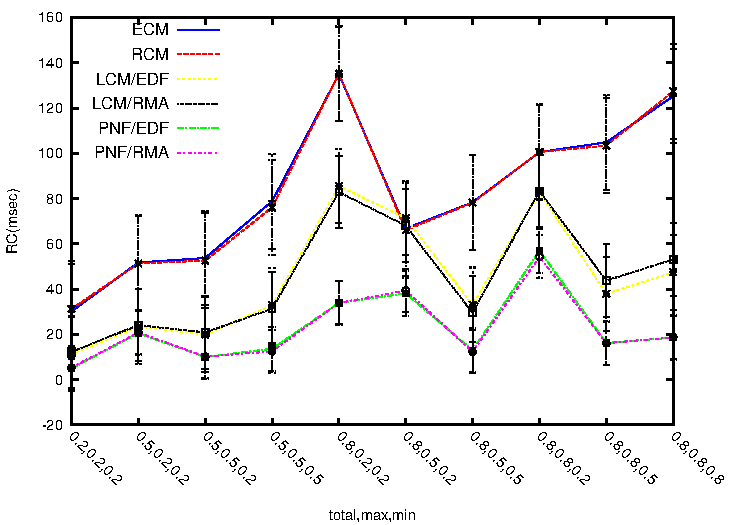
\includegraphics[scale=0.7]
{figures/Abr_dur_4t_100obj_80wr}
\label{fig:4t_ecm_rcm_lcm_pnf_100obj_80wr}
}
~
\subfigure[8 tasks]{
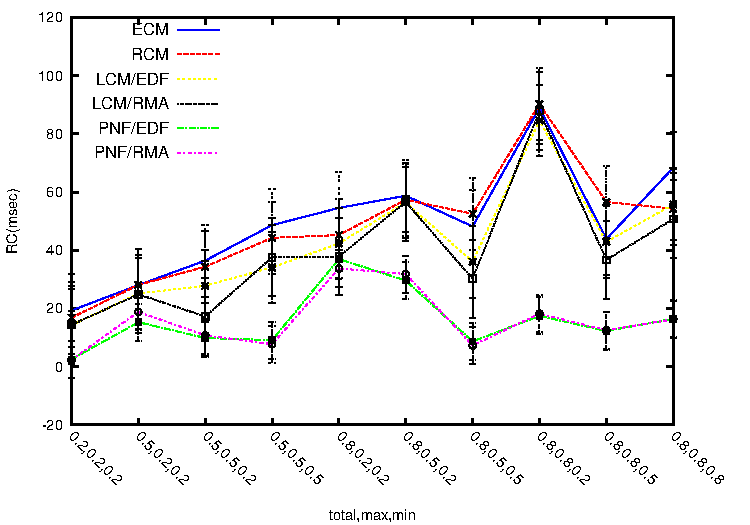
\includegraphics[scale=0.7]
{figures/Abr_dur_8t_180obj_80wr}
\label{fig:8t_ecm_rcm_lcm_pnf_180obj_80wr}
}
~
\subfigure[20 tasks]{
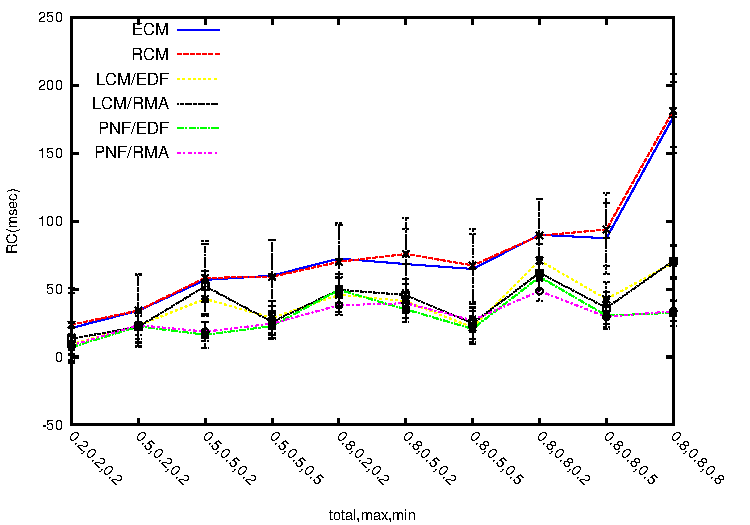
\includegraphics[scale=0.7]
{figures/Abr_dur_20t_420obj_80wr}
\label{fig:20t_ecm_rcm_lcm_pnf_420obj_80wr}
}
\caption{Average retry cost for 40 objects per transaction, 80\% write operations for different values of total, maximum and minimum atomic section length under different CMs}
\label{fig:cm_40obj_per_tx_80wr}
\end{figure}
%%%%%%%%%%%%%%%%%%%%%%%%%%%%%%%%%%%%%%%%%%%%%%%%%%%%%%
\begin{figure}
\centering

\subfigure[4 tasks]{
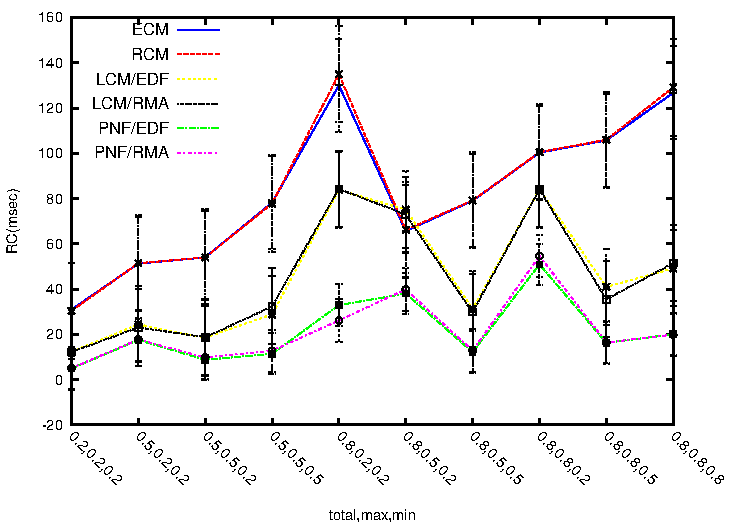
\includegraphics[scale=0.7]
{figures/Abr_dur_4t_100obj_100wr}
\label{fig:4t_ecm_rcm_lcm_pnf_100obj_100wr}
}
~
\subfigure[8 tasks]{
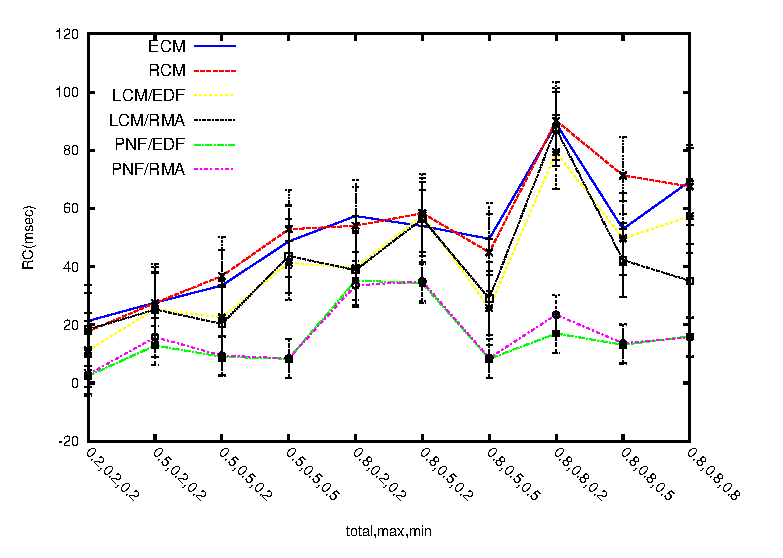
\includegraphics[scale=0.7]
{figures/Abr_dur_8t_180obj_100wr}
\label{fig:8t_ecm_rcm_lcm_pnf_180obj_100wr}
}
~
\subfigure[20 tasks]{
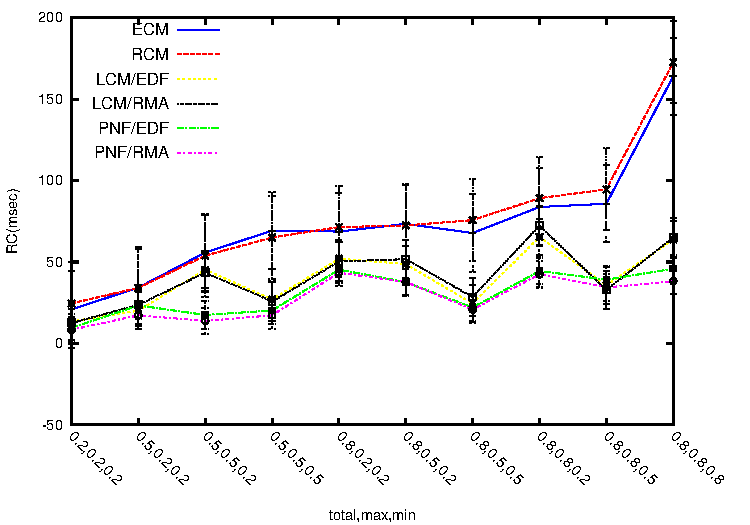
\includegraphics[scale=0.7]
{figures/Abr_dur_20t_420obj_100wr}
\label{fig:20t_ecm_rcm_lcm_pnf_420obj_100wr}
}
\caption{Average retry cost for 40 objects per transaction, 100\% write operations for different values of total, maximum and minimum atomic section length under different CMs}
\label{fig:cm_40obj_per_tx_100wr}
\end{figure}